% compile with pdflatex slides.tex

\documentclass{beamer}
\usepackage[utf8]{inputenc}

% \usepackage{pgfpages}
% \pgfpagesuselayout{4 on 1}[a4paper,landscape,border shrink=5mm]

\usepackage{graphicx}

\usepackage{color}

\usepackage{beamerthemesplit}
\usetheme{progressbar}

\usepackage{tikz}
\usetikzlibrary{shapes}
\usetikzlibrary{arrows,decorations.pathmorphing,backgrounds,positioning,fit}
\tikzset{terminal node/.style={circle, draw,
    rounded corners, shade, top color=white, bottom 
    color=blue!50!black!20, draw=blue!40!black!60, thick}}
\tikzset{mdd node/.style={terminal node, rectangle split, rectangle split horizontal, rectangle split parts=#1}}
\tikzset{regular edge/.style={draw=blue!40!black!60, thick}}
\tikzset{outgoing edge/.style={regular edge, very thin}}
\tikzset{comment/.style={blue!95}}
\tikzset{diagram background/.style={fill=blue!2,rounded corners=0.5cm}}

\renewcommand{\O}{\mathrm{O}}
\newcommand{\Z}{\mathbb{Z}}

\title{Model checking with edge-valued decision diagrams}

\institute{
  École Normale Supérieure de Lyon, France
  (\texttt{pierre.roux@ens-lyon.fr})
  \and
  NIA
  (\texttt{radu@nianet.org})
}

\author{
  Pierre~Roux\inst{1}
  \and
  Radu~I.~Siminiceanu\inst{2}
}

%\date{}

\everymath{\displaystyle}

%\includeonlyframes{current}

\begin{document}

\frame{
  \titlepage
}

\frame{\tableofcontents}

%% \AtBeginSection[] 
%% {
%% \begin{frame}<beamer>
%%   \tableofcontents[currentsection]
%% \end{frame}
%% }

\section{BDD and ADD}

\begin{frame}
  \frametitle{Model Checking}
  \vspace{-3.2cm}
  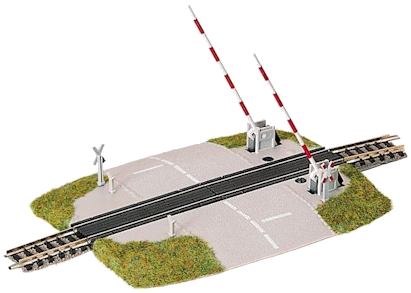
\includegraphics[width=11cm]{railroad_crossing}
  \vspace{-8.2cm}
  \begin{itemize}
  \item States in $\left\{train_l, no\_train_l\right\} \times \left\{barrier\_up, barrier\_down\right\} \times \left\{train_r, no\_train_r\right\}$
  \item Transition relation
    \begin{itemize}
    \item $train_l \rightarrow barrier\_down$
    \item ...
    \end{itemize}
  \end{itemize}
\end{frame}

\begin{frame}
  \frametitle{Representation of functions}
  For Model Checking we need to represent
  \begin{itemize}
  \item Boolean functions $f : \left\{0, 1\right\}^n \rightarrow \left\{0, 1\right\}$
  \item sets $\left\{x \in \left\{0, 1\right\}^n \;|\; f(x) = 1\right\}$
  \end{itemize}
  \pause
  First idea: truth table
  $$
  \begin{array}{ccc|c}
    a & b & c & f(a, b, c) \\
    \hline
    0 & 0 & 0 & 0 \\
    0 & 0 & 1 & 1 \\
    0 & 1 & 0 & 0 \\
    0 & 1 & 1 & 1 \\
    1 & 0 & 0 & 1 \\
    1 & 0 & 1 & 0 \\
    1 & 1 & 0 & 0 \\
    1 & 1 & 1 & 1
  \end{array}
  $$
  \pause
  \alert{requires $2^n$ entries}
\end{frame}

\begin{frame}
  \frametitle{Trees}
  Second idea: using trees
  \vspace{-0.5cm}
  \begin{center}
    \hspace{-0.5cm}
    \begin{tikzpicture}
      [xscale=0.75, yscale=1.8, auto]
      \node [mdd node=3]    (l3n0)    at ( 0, 3) {$a$\nodepart{two}0\nodepart{three}1};
      \node [mdd node=3]    (l2n0)    at (-4, 2) {$b$\nodepart{two}0\nodepart{three}1};
      \node [mdd node=3]    (l2n1)    at ( 4, 2) {$b$\nodepart{two}0\nodepart{three}1};
      \node [mdd node=3]    (l1n0)    at (-6, 1) {$c$\nodepart{two}0\nodepart{three}1};
      \node [mdd node=3]    (l1n1)    at (-2, 1) {$c$\nodepart{two}0\nodepart{three}1};
      \node [mdd node=3]    (l1n2)    at ( 2, 1) {$c$\nodepart{two}0\nodepart{three}1};
      \node [mdd node=3]    (l1n3)    at ( 6, 1) {$c$\nodepart{two}0\nodepart{three}1};
      \node [terminal node] (bottom0) at (-7, 0) {0};
      \node [terminal node] (bottom1) at (-5, 0) {1};
      \node [terminal node] (bottom2) at (-3, 0) {0};
      \node [terminal node] (bottom3) at (-1, 0) {1};
      \node [terminal node] (bottom4) at ( 1, 0) {1};
      \node [terminal node] (bottom5) at ( 3, 0) {0};
      \node [terminal node] (bottom6) at ( 5, 0) {0};
      \node [terminal node] (bottom7) at ( 7, 0) {1};
      
      \draw [regular edge]  (l3n0.two   |- l3n0.south) to (l2n0);
      \draw [regular edge]  (l3n0.three |- l3n0.south) to (l2n1);
      \draw [regular edge]  (l2n0.two   |- l2n0.south) to (l1n0);
      \draw [regular edge]  (l2n0.three |- l2n0.south) to (l1n1);
      \draw [regular edge]  (l2n1.two   |- l2n1.south) to (l1n2);
      \draw [regular edge]  (l2n1.three |- l2n1.south) to (l1n3);
      \draw [regular edge]  (l1n0.two   |- l1n0.south) to (bottom0);
      \draw [regular edge]  (l1n0.three |- l1n0.south) to (bottom1);
      \draw [regular edge]  (l1n1.two   |- l1n1.south) to (bottom2);
      \draw [regular edge]  (l1n1.three |- l1n1.south) to (bottom3);
      \draw [regular edge]  (l1n2.two   |- l1n2.south) to (bottom4);
      \draw [regular edge]  (l1n2.three |- l1n2.south) to (bottom5);
      \draw [regular edge]  (l1n3.two   |- l1n3.south) to (bottom6);
      \draw [regular edge]  (l1n3.three |- l1n3.south) to (bottom7);
    \end{tikzpicture}
  \end{center}
  \pause
  \alert{still requires $2^n$ terminal nodes}
\end{frame}

\begin{frame}
  \frametitle{Binary Decision Diagram (BDD)}
  \vspace{-0.13cm}
  Merging terminal nodes
  \vspace{-0.5cm}
  \begin{center}
    \hspace{-0.53cm}
    \begin{tikzpicture}
      [xscale=0.75, yscale=1.8, auto]
      \node     [mdd node=3]    (l3n0)    at ( 0, 3) {$a$\nodepart{two}0\nodepart{three}1};
      \node     [mdd node=3]    (l2n0)    at (-4, 2) {$b$\nodepart{two}0\nodepart{three}1};
      \node     [mdd node=3]    (l2n1)    at ( 4, 2) {$b$\nodepart{two}0\nodepart{three}1};
      \node     [mdd node=3]    (l1n0)    at (-6, 1) {$c$\nodepart{two}0\nodepart{three}1};
      \node     [mdd node=3]    (l1n1)    at (-2, 1) {$c$\nodepart{two}0\nodepart{three}1};
      \node     [mdd node=3]    (l1n2)    at ( 2, 1) {$c$\nodepart{two}0\nodepart{three}1};
      \node     [mdd node=3]    (l1n3)    at ( 6, 1) {$c$\nodepart{two}0\nodepart{three}1};
      \node<1>  [terminal node] (bottom0) at (-7, 0) {0};
      \node<1>  [terminal node] (bottom1) at (-5, 0) {1};
      \node<1>  [terminal node] (bottom2) at (-3, 0) {0};
      \node<1>  [terminal node] (bottom3) at (-1, 0) {1};
      \node<1>  [terminal node] (bottom4) at ( 1, 0) {1};
      \node<1>  [terminal node] (bottom5) at ( 3, 0) {0};
      \node<1>  [terminal node] (bottom6) at ( 5, 0) {0};
      \node<1>  [terminal node] (bottom7) at ( 7, 0) {1};
      \node<2-> [terminal node] (bottom0) at (-2, 0) {0};
      \node<2-> [terminal node] (bottom1) at ( 2, 0) {1};

      \draw     [regular edge]  (l3n0.two   |- l3n0.south) to (l2n0);
      \draw     [regular edge]  (l3n0.three |- l3n0.south) to (l2n1);
      \draw     [regular edge]  (l2n0.two   |- l2n0.south) to (l1n0);
      \draw     [regular edge]  (l2n0.three |- l2n0.south) to (l1n1);
      \draw     [regular edge]  (l2n1.two   |- l2n1.south) to (l1n2);
      \draw     [regular edge]  (l2n1.three |- l2n1.south) to (l1n3);
      \draw<1>  [regular edge]  (l1n0.two   |- l1n0.south) to (bottom0);
      \draw<1>  [regular edge]  (l1n0.three |- l1n0.south) to (bottom1);
      \draw<1>  [regular edge]  (l1n1.two   |- l1n1.south) to (bottom2);
      \draw<1>  [regular edge]  (l1n1.three |- l1n1.south) to (bottom3);
      \draw<1>  [regular edge]  (l1n2.two   |- l1n2.south) to (bottom4);
      \draw<1>  [regular edge]  (l1n2.three |- l1n2.south) to (bottom5);
      \draw<1>  [regular edge]  (l1n3.two   |- l1n3.south) to (bottom6);
      \draw<1>  [regular edge]  (l1n3.three |- l1n3.south) to (bottom7);
      \draw<2-> [regular edge]  (l1n0.two   |- l1n0.south) to (bottom0);
      \draw<2-> [regular edge]  (l1n0.three |- l1n0.south) to (bottom1);
      \draw<2-> [regular edge]  (l1n1.two   |- l1n1.south) to (bottom0);
      \draw<2-> [regular edge]  (l1n1.three |- l1n1.south) to (bottom1);
      \draw<2-> [regular edge]  (l1n2.two   |- l1n2.south) to (bottom1);
      \draw<2-> [regular edge]  (l1n2.three |- l1n2.south) to (bottom0);
      \draw<2-> [regular edge]  (l1n3.two   |- l1n3.south) to (bottom0);
      \draw<2-> [regular edge]  (l1n3.three |- l1n3.south) to (bottom1);
    \end{tikzpicture}
  \end{center}
  \visible<3>{still exponential}
  \transdissolve<2>[duration=2]
\end{frame}

\begin{frame}
  \frametitle{BDD cont'd}
  Merging duplicate nodes
  \vspace{-0.5cm}
  \begin{center}
    \hspace{-0.53cm}
    \begin{tikzpicture}
      [xscale=0.75, yscale=1.8, auto]
      \node     [mdd node=3]    (l3n0)    at ( 0, 3) {$a$\nodepart{two}0\nodepart{three}1};
      \node     [mdd node=3]    (l2n0)    at (-4, 2) {$b$\nodepart{two}0\nodepart{three}1};
      \node     [mdd node=3]    (l2n1)    at ( 4, 2) {$b$\nodepart{two}0\nodepart{three}1};
      \node<1>  [mdd node=3]    (l1n0)    at (-6, 1) {$c$\nodepart{two}0\nodepart{three}1};
      \node     [mdd node=3]    (l1n1)    at (-2, 1) {$c$\nodepart{two}0\nodepart{three}1};
      \node     [mdd node=3]    (l1n2)    at ( 2, 1) {$c$\nodepart{two}0\nodepart{three}1};
      \node<1>  [mdd node=3]    (l1n3)    at ( 6, 1) {$c$\nodepart{two}0\nodepart{three}1};
      \node     [terminal node] (bottom0) at (-2, 0) {0};
      \node     [terminal node] (bottom1) at ( 2, 0) {1};

      \draw     [regular edge]  (l3n0.two   |- l3n0.south) to (l2n0);
      \draw     [regular edge]  (l3n0.three |- l3n0.south) to (l2n1);
      \draw<1>  [regular edge]  (l2n0.two   |- l2n0.south) to (l1n0);
      \draw<2-> [regular edge]  (l2n0.two   |- l2n0.south) to (l1n1);
      \draw     [regular edge]  (l2n0.three |- l2n0.south) to (l1n1);
      \draw     [regular edge]  (l2n1.two   |- l2n1.south) to (l1n2);
      \draw<1>  [regular edge]  (l2n1.three |- l2n1.south) to (l1n3);
      \draw<2-> [regular edge]  (l2n1.three |- l2n1.south) to (l1n1);
      \draw<1>  [regular edge]  (l1n0.two   |- l1n0.south) to (bottom0);
      \draw<1>  [regular edge]  (l1n0.three |- l1n0.south) to (bottom1);
      \draw     [regular edge]  (l1n1.two   |- l1n1.south) to (bottom0);
      \draw     [regular edge]  (l1n1.three |- l1n1.south) to (bottom1);
      \draw     [regular edge]  (l1n2.two   |- l1n2.south) to (bottom1);
      \draw     [regular edge]  (l1n2.three |- l1n2.south) to (bottom0);
      \draw<1>  [regular edge]  (l1n3.two   |- l1n3.south) to (bottom0);
      \draw<1>  [regular edge]  (l1n3.three |- l1n3.south) to (bottom1);
    \end{tikzpicture}
  \end{center}
  \visible<3>{exponential in worst case, often better in practice}
  \transdissolve<2>[duration=2]
\end{frame}

\begin{frame}
  \frametitle{BDD end}
  Deleting redundant nodes
  \vspace{-0.5cm}
  \begin{center}
    \hspace{-0.53cm}
    \begin{tikzpicture}
      [xscale=0.75, yscale=1.8, auto]
      \node     [mdd node=3]    (l3n0)    at ( 0, 3) {$a$\nodepart{two}0\nodepart{three}1};
      \visible<1>{
        \node   [mdd node=3]    (l2n0)    at (-4, 2) {$b$\nodepart{two}0\nodepart{three}1};
      }
      \node     [mdd node=3]    (l2n1)    at ( 4, 2) {$b$\nodepart{two}0\nodepart{three}1};
      \node     [mdd node=3]    (l1n1)    at (-2, 1) {$c$\nodepart{two}0\nodepart{three}1};
      \node     [mdd node=3]    (l1n2)    at ( 2, 1) {$c$\nodepart{two}0\nodepart{three}1};
      \node     [terminal node] (bottom0) at (-2, 0) {0};
      \node     [terminal node] (bottom1) at ( 2, 0) {1};

      \draw<1>  [regular edge]  (l3n0.two   |- l3n0.south) to (l2n0);
      \draw<2-> [regular edge]  (l3n0.two   |- l3n0.south) to (l1n1);
      \draw     [regular edge]  (l3n0.three |- l3n0.south) to (l2n1);
      \draw<1>  [regular edge]  (l2n0.two   |- l2n0.south) to (l1n1);
      \draw<1>  [regular edge]  (l2n0.three |- l2n0.south) to (l1n1);
      \draw     [regular edge]  (l2n1.two   |- l2n1.south) to (l1n2);
      \draw     [regular edge]  (l2n1.three |- l2n1.south) to (l1n1);
      \draw     [regular edge]  (l1n1.two   |- l1n1.south) to (bottom0);
      \draw     [regular edge]  (l1n1.three |- l1n1.south) to (bottom1);
      \draw     [regular edge]  (l1n2.two   |- l1n2.south) to (bottom1);
      \draw     [regular edge]  (l1n2.three |- l1n2.south) to (bottom0);
    \end{tikzpicture}
  \end{center}
  \visible<3>{less important but still interesting}
  \transdissolve<2>[duration=2]
\end{frame}

\begin{frame}
  \frametitle{BDD characteristics}
  \begin{itemize}
  \item canonicity:\\
    two BDD represent the same function iff they are isomorphic
  \item easy computation:\\
    for $f$, $g$ represented by BDDs of size $|f|$ and $|g|$\\
    $f*g$ computed in $\O\left(|f|\,|g|\right)$
  \end{itemize}
\end{frame}

\begin{frame}
  \frametitle{ADD}
  \begin{itemize}
  \item $f : \left\{0, 1\right\}^n \rightarrow \alert<1>{\Z}$
    \pause
  \item Extend BDD to \alert<2>{Multiple Terminal BDD}
    {\normalsize
    \begin{center}
      \begin{figure}
        \begin{tikzpicture}
          [xscale=1, yscale=1.5, auto]
          \node [mdd node=3]    (l3n0)    at ( 0, 2) {$a$\nodepart{two}0\nodepart{three}1};
          \node [mdd node=3]    (l2n0)    at (-2, 1) {$b$\nodepart{two}0\nodepart{three}1};
          \node [mdd node=3]    (l2n1)    at ( 2, 1) {$b$\nodepart{two}0\nodepart{three}1};
          \node [terminal node] (bottom0) at (-3, 0) {0};
          \node [terminal node] (bottom1) at (-1, 0) {1};
          \node [terminal node] (bottom2) at ( 1, 0) {2};
          \node [terminal node] (bottom3) at ( 3, 0) {3};
          
          \draw [regular edge]  (l3n0.two   |- l3n0.south) to (l2n0);
          \draw [regular edge]  (l3n0.three |- l3n0.south) to (l2n1);
          \draw [regular edge]  (l2n0.two   |- l2n0.south) to (bottom0);
          \draw [regular edge]  (l2n0.three |- l2n0.south) to (bottom1);
          \draw [regular edge]  (l2n1.two   |- l2n1.south) to (bottom2);
          \draw [regular edge]  (l2n1.three |- l2n1.south) to (bottom3);
        \end{tikzpicture}
        \caption{$f : (a, b) \mapsto 2a+b$}
      \end{figure}
    \end{center}}
    \pause
  \item Bad if $\mathrm{Img}\left(f\right)$ too big
  \end{itemize}
\end{frame}

\section{EVMDD}

\begin{frame}
  \frametitle{Edge Valued MDD (EVMDD)}
  \vspace{0.26cm}
  Merging all terminals to 0 and putting values on edges
  \begin{center}
    \hspace{0.52cm}
    \begin{tikzpicture}
      [xscale=1, yscale=1.5, auto]
      \node     [mdd node=3]    (l3n0)     at ( 0, 2) {$a$\nodepart{two}0\nodepart{three}1};
      \node     [mdd node=3]    (l2n0)     at (-2, 1) {$b$\nodepart{two}0\nodepart{three}1};
      \node     [mdd node=3]    (l2n1)     at ( 2, 1) {$b$\nodepart{two}0\nodepart{three}1};
      \node<1>  [terminal node] (bottom0)  at (-3, 0) {0};
      \node<1>  [terminal node] (bottom1)  at (-1, 0) {1};
      \node<1>  [terminal node] (bottom2)  at ( 1, 0) {2};
      \node<1>  [terminal node] (bottom3)  at ( 3, 0) {3};
      \node<2-> [terminal node] (bottomv0) at ( 0, 0) {0};
      
      \draw<1>  [regular edge]  (l3n0.two   |- l3n0.south) to                 (l2n0);
      \draw<1>  [regular edge]  (l3n0.three |- l3n0.south) to                 (l2n1);
      \draw<2-> [regular edge]  (l3n0.two   |- l3n0.south) to node [swap] {0} (l2n0);
      \draw<2-> [regular edge]  (l3n0.three |- l3n0.south) to node        {0} (l2n1);
      \draw<1>  [regular edge]  (l2n0.two   |- l2n0.south) to                 (bottom0);
      \draw<1>  [regular edge]  (l2n0.three |- l2n0.south) to                 (bottom1);
      \draw<1>  [regular edge]  (l2n1.two   |- l2n1.south) to                 (bottom2);
      \draw<1>  [regular edge]  (l2n1.three |- l2n1.south) to                 (bottom3);
      \draw<2-> [regular edge]  (l2n0.two   |- l2n0.south) to node [swap] {0} (bottomv0);
      \draw<2-> [regular edge]  (l2n0.three |- l2n0.south) to node        {1} (bottomv0);
      \draw<2-> [regular edge]  (l2n1.two   |- l2n1.south) to node [swap] {2} (bottomv0);
      \draw<2-> [regular edge]  (l2n1.three |- l2n1.south) to node        {3} (bottomv0);
    \end{tikzpicture}
  \end{center}
  \visible<3->{Result: sum of edge values on path from root to terminal node}\\
  \visible<4>{still not better...}  
  \transdissolve<2>[duration=2]
\end{frame}

\begin{frame}
  \frametitle{EVMDD cont'd}
  \vspace{0.06cm}
  Canonical node: minimum of outgoing edge values is 0
  \begin{center}
    \hspace{0.52cm}
    \begin{tikzpicture}
      [xscale=1, yscale=1.5, auto]
      \node     [mdd node=3]    (l3n0)     at ( 0, 2) {$a$\nodepart{two}0\nodepart{three}1};
      \node     [mdd node=3]    (l2n0)     at (-2, 1) {$b$\nodepart{two}0\nodepart{three}1};
      \node     [mdd node=3]    (l2n1)     at ( 2, 1) {$b$\nodepart{two}0\nodepart{three}1};
      \node     [terminal node] (bottomv0) at ( 0, 0) {0};
      
      \draw     [regular edge]  (l3n0.two   |- l3n0.south) to node [swap] {0} (l2n0);
      \draw<1>  [regular edge]  (l3n0.three |- l3n0.south) to node        {0} (l2n1);
      \draw<2-> [regular edge]  (l3n0.three |- l3n0.south) to node        {2} (l2n1);
      \draw     [regular edge]  (l2n0.two   |- l2n0.south) to node [swap] {0} (bottomv0);
      \draw     [regular edge]  (l2n0.three |- l2n0.south) to node        {1} (bottomv0);
      \draw<1>  [regular edge]  (l2n1.two   |- l2n1.south) to node [swap] {2} (bottomv0);
      \draw<1>  [regular edge]  (l2n1.three |- l2n1.south) to node        {3} (bottomv0);
      \draw<2-> [regular edge]  (l2n1.two   |- l2n1.south) to node [swap] {0} (bottomv0);
      \draw<2-> [regular edge]  (l2n1.three |- l2n1.south) to node        {1} (bottomv0);
    \end{tikzpicture}
  \end{center}
  \visible<3>{still not better...}  
  \transdissolve<2>[duration=2]
\end{frame}

\begin{frame}
  \frametitle{EVMDD end}
  \vspace{0.11cm}
  Merging duplicate nodes
  \begin{center}
    \hspace{0.52cm}
    \begin{tikzpicture}
      [xscale=1, yscale=1.5, auto]
      \node     [mdd node=3]    (l3n0)     at ( 0, 2) {$a$\nodepart{two}0\nodepart{three}1};
      \node     [mdd node=3]    (l2n0)     at (-2, 1) {$b$\nodepart{two}0\nodepart{three}1};
      \visible<1>{
        \node   [mdd node=3]    (l2n1)     at ( 2, 1) {$b$\nodepart{two}0\nodepart{three}1};
      }
      \node     [terminal node] (bottomv0) at ( 0, 0) {0};
      
      \draw     [regular edge]  (l3n0.two   |- l3n0.south) to node [swap] {0} (l2n0);
      \draw<1>  [regular edge]  (l3n0.three |- l3n0.south) to node        {2} (l2n1);
      \draw<2-> [regular edge]  (l3n0.three |- l3n0.south) to node        {2} (l2n0);
      \draw     [regular edge]  (l2n0.two   |- l2n0.south) to node [swap] {0} (bottomv0);
      \draw     [regular edge]  (l2n0.three |- l2n0.south) to node        {1} (bottomv0);
      \draw<1>  [regular edge]  (l2n1.two   |- l2n1.south) to node [swap] {0} (bottomv0);
      \draw<1>  [regular edge]  (l2n1.three |- l2n1.south) to node        {1} (bottomv0);
    \end{tikzpicture}
  \end{center}
  \visible<3>{\alert{here we can gain}}  
  \transdissolve<2>[duration=2]
\end{frame}

\begin{frame}
  \frametitle{EVMDD characteristics}
  \begin{itemize}
  \item We proved EVMDD cannot be bigger than ADD
  \item Very good for linear functions (only one node per level)
  \item computation: we wrote an algorithm\\
    for $f$, $g$ represented by EVMDDs of size $|f|$ and $|g|$\\
    $f*g$ computed in $\O\left(|f|\,|g|\,|\mathrm{Img}(f)|\,|\mathrm{Img}(g)|\right)$
  \item We proved this algorithm has \alert{exactly the same complexity}\\
    as its equivalent for BDD, hence not any gain
  \item Can we do better ?
  \end{itemize}
\end{frame}

\begin{frame}
  \frametitle{EVMDD algorithms}
  Yes for following operations
  \begin{itemize}
  \item Addition:\\
    $f+g$ computed in $\O\left(|f|\,|g|\right)$
  \item Multiplication:\\
    $f\times g$ computed in $\O\left(|f|^2\,|g|^2\,|f\times g|\right)$
    \begin{itemize}
    \item seems far better on some examples
    \item not any theoretic proof of that yet
    \end{itemize}
  \item Adding constant:\\
    $f+c$ computed in $\O(1)$
  \item Multiplication by constant:\\
    $f\times c$ computed in $\O(|f|)$
  \item Division or modulo constant:\\
    $f/c$ and $f\%c$ computed in $\O(|f|c)$
  \end{itemize}
\end{frame}

\section{Implementation}

\begin{frame}
  \frametitle{Our implementation}
  Featuring
  \begin{itemize}
  \item EVMDD for arithmetic expressions
  \item MDD for boolean expressions
  \item Breadth First Search and Saturation based state space construction
  \item identity reduced transition relations
  \end{itemize}
  Some metrics
  \begin{itemize}
  \item less than 4800 lines of ANSI C code for library
  \item 8500 lines for the entire little model checker
  \end{itemize}
\end{frame}

\begin{frame}
  \frametitle{Implementation choices}
  \begin{itemize}
  \item node indexing
    \begin{itemize}
    \item pointers
    \item couple $(level, index)$
    \end{itemize}
    \pause
  \item reduction
    \begin{itemize}
    \item quasi reduced
    \item fully reduced
    \item identity reduced
    \end{itemize}
    \pause
  \item caching
    \begin{itemize}
    \item lossy
    \item hash tables with chaining
    \end{itemize}
    \pause
  \item garbage collection
    \begin{itemize}
    \item reference counting
    \item mark \& sweep
    \item stop \& copy
    \end{itemize}
  \end{itemize}
\end{frame}

\begin{frame}
  \frametitle{Demo}
  EVMDD can be dramatically more efficient than ADD
% src/evmdd -v --cudd < test0
% src/evmdd -v < test0
% src/evmdd -v < test2
\end{frame}

\begin{frame}
  \frametitle{Demo cont'd}
  Dining philosophers
  \vspace{-0.5cm}
  \begin{center}
    \hspace{3.5cm}
    \begin{tikzpicture}
      % table
      \fill [brown]                   (0, 0) circle (2.2cm);
      \foreach \angle/\maincolor/\haircolor in {0/red/yellow, 90/green/black, 180/blue/brown, 270/yellow/brown!60!black} {
        % hilosophers
        \fill [rotate=\angle, \maincolor, rounded corners=0.2cm] (3cm, 0cm) ++(-0.25cm, -0.8cm) rectangle ++(0.5cm, 1.6cm);
        \fill [rotate=\angle, \haircolor] (3cm, 0cm) circle (0.4cm);
        % plates
        \fill [rotate=\angle, white] (1.5cm, 0cm) circle (0.6cm);
        \draw [rotate=\angle, black!40] (1.5cm, 0cm) circle (0.4cm);
        % forks
        \fill [rotate=\angle, rotate=45, white!40!black, rounded corners] (1.2cm, 0cm) ++(0cm, -0.15cm) rectangle ++(0.8cm, 0.3cm);
        \fill [rotate=\angle, rotate=45, white!40!black] (1.1cm, 0cm) ++(0cm, -0.2cm) rectangle ++(0.2cm, 0.4cm);
        \foreach \offset in {-0.25cm, -0.05cm, 0.15cm}
        \fill [rotate=\angle, rotate=45, white!40!black, rounded corners=0.05cm] (0.8cm, 0cm) ++(0cm, \offset) rectangle ++(0.5cm, 0.1cm);
      }
    \end{tikzpicture}\\
    \vspace{-5cm}
    \hspace{-8cm}
    \begin{tikzpicture}
      [yscale=1.5]
      \node (ff) at (0, 1) {fork free};
      \node (fu) at (0, 0) {fork used};

      \draw [->] (ff) to [out=235, in=135] (fu);
      \draw [->] (fu) to [out=45, in=315] (ff);
    \end{tikzpicture}\\
    \vspace{1.5cm}
    \hspace{-6cm}
    \begin{tikzpicture}
      [xscale=2, yscale=0.4]
      \node (waiting) at (-1, 0) {waiting};
      \node (fl)      at ( 0, 1) {fork left};
      \node (fr)      at ( 0,-1) {fork right};
      \node [yshift=-0.4cm] (anchor)  at ( 0,-2) {};
      \node (eating)  at ( 1, 0) {eating};

      \draw [->] (waiting) to (fl.west);
      \draw [->] (waiting) to (fr.west);
      \draw [->] (fl.east)      to (eating);
      \draw [->] (fr.east)      to (eating);
      \draw (eating.south)  to [out=270, in=0] (anchor.center);
      \draw [->] (anchor.center)  to [out=180, in=270] (waiting.south);
    \end{tikzpicture}
  \end{center}
\end{frame}

\begin{frame}
  \frametitle{Demo cont'd}
  Dining philosophers, results
  \begin{table}
    \begin{tabular}{r|ccc}
      nb of phils & CUDD & saturation & with identity reduction \\
      \hline
      10 & 0.012 & 0.020 & 0.000 \\
      50 & 0.220 & 0.352 & 0.016 \\
      100 & 0.856 & 1.700 & 0.028 \\
      1000 & - & - & 0.984
    \end{tabular}
    \caption{Building transition relation (in s)}
  \end{table}

  \begin{table}
    \begin{tabular}{r|ccc}
      nb of phils & CUDD & saturation & with identity reduction \\
      \hline
      10 & 0.032 & 0.004 & 0.000 \\
      50 & 0.952 & 0.004 & 0.004 \\
      100 & 5.372 & 0.008 & 0.008 \\
      1000 & - & - & 0.092
    \end{tabular}
    \caption{Computing state space (in s)}
  \end{table}
\end{frame}

\begin{frame}[label=current]
  \frametitle{Demo end}   
  Knights
  \begin{tikzpicture}
    [scale=0.9]
    \begin{scope}
      \fill [white] (0, 0) rectangle ++(1, 1);
      \fill [black] (1, 0) rectangle ++(1, 1);
      \fill [white] (2, 0) rectangle ++(1, 1);
      \fill [black] (3, 0) rectangle ++(1, 1);
      \fill [white] (4, 0) rectangle ++(1, 1);
      \fill [black] (0, 1) rectangle ++(1, 1);
      \fill [white] (1, 1) rectangle ++(1, 1);
      \fill [black] (2, 1) rectangle ++(1, 1);
      \fill [white] (3, 1) rectangle ++(1, 1);
      \fill [black] (4, 1) rectangle ++(1, 1);
      \fill [white] (0, 2) rectangle ++(1, 1);
      \fill [black] (1, 2) rectangle ++(1, 1);
      \fill [white] (2, 2) rectangle ++(1, 1);
      \fill [black] (3, 2) rectangle ++(1, 1);
      \fill [white] (4, 2) rectangle ++(1, 1);
      \fill [black] (0, 3) rectangle ++(1, 1);
      \fill [white] (1, 3) rectangle ++(1, 1);
      \fill [black] (2, 3) rectangle ++(1, 1);
      \fill [white] (3, 3) rectangle ++(1, 1);
      \fill [black] (4, 3) rectangle ++(1, 1);
      \fill [white] (0, 4) rectangle ++(1, 1);
      \fill [black] (1, 4) rectangle ++(1, 1);
      \fill [white] (2, 4) rectangle ++(1, 1);
      \fill [black] (3, 4) rectangle ++(1, 1);
      \fill [white] (4, 4) rectangle ++(1, 1);

      \node (b00) at (0.5, 0.5) {
\includegraphics[width=0.8cm]{black_knight}};
      \node       at (1.5, 0.5) {
\includegraphics[width=0.8cm]{white_knight}};
      \node       at (2.5, 0.5) {
\includegraphics[width=0.8cm]{white_knight}};
      \node       at (3.5, 0.5) {
\includegraphics[width=0.8cm]{white_knight}};
      \node       at (4.5, 0.5) {
\includegraphics[width=0.8cm]{white_knight}};
      \node       at (0.5, 1.5) {
\includegraphics[width=0.8cm]{black_knight}};
      \node       at (1.5, 1.5) {
\includegraphics[width=0.8cm]{black_knight}};
      \node       at (2.5, 1.5) {
\includegraphics[width=0.8cm]{white_knight}};
      \node       at (3.5, 1.5) {
\includegraphics[width=0.8cm]{white_knight}};
      \node       at (4.5, 1.5) {
\includegraphics[width=0.8cm]{white_knight}};
      \node       at (0.5, 2.5) {
\includegraphics[width=0.8cm]{black_knight}};
      \node       at (1.5, 2.5) {
\includegraphics[width=0.8cm]{black_knight}};
      % free cell
      \node       at (3.5, 2.5) {
\includegraphics[width=0.8cm]{white_knight}};
      \node       at (4.5, 2.5) {
\includegraphics[width=0.8cm]{white_knight}};
      \node       at (0.5, 3.5) {
\includegraphics[width=0.8cm]{black_knight}};
      \node       at (1.5, 3.5) {
\includegraphics[width=0.8cm]{black_knight}};
      \node       at (2.5, 3.5) {
\includegraphics[width=0.8cm]{black_knight}};
      \node       at (3.5, 3.5) {
\includegraphics[width=0.8cm]{white_knight}};
      \node       at (4.5, 3.5) {
\includegraphics[width=0.8cm]{white_knight}};
      \node       at (0.5, 4.5) {
\includegraphics[width=0.8cm]{black_knight}};
      \node       at (1.5, 4.5) {
\includegraphics[width=0.8cm]{black_knight}};
      \node       at (2.5, 4.5) {
\includegraphics[width=0.8cm]{black_knight}};
      \node       at (3.5, 4.5) {
\includegraphics[width=0.8cm]{black_knight}};
      \node (b44) at (4.5, 4.5) {
\includegraphics[width=0.8cm]{white_knight}};
    \end{scope}

    \begin{scope}[xshift=6.5cm]
      \fill [white] (0, 0) rectangle ++(1, 1);
      \fill [black] (1, 0) rectangle ++(1, 1);
      \fill [white] (2, 0) rectangle ++(1, 1);
      \fill [black] (3, 0) rectangle ++(1, 1);
      \fill [white] (4, 0) rectangle ++(1, 1);
      \fill [black] (0, 1) rectangle ++(1, 1);
      \fill [white] (1, 1) rectangle ++(1, 1);
      \fill [black] (2, 1) rectangle ++(1, 1);
      \fill [white] (3, 1) rectangle ++(1, 1);
      \fill [black] (4, 1) rectangle ++(1, 1);
      \fill [white] (0, 2) rectangle ++(1, 1);
      \fill [black] (1, 2) rectangle ++(1, 1);
      \fill [white] (2, 2) rectangle ++(1, 1);
      \fill [black] (3, 2) rectangle ++(1, 1);
      \fill [white] (4, 2) rectangle ++(1, 1);
      \fill [black] (0, 3) rectangle ++(1, 1);
      \fill [white] (1, 3) rectangle ++(1, 1);
      \fill [black] (2, 3) rectangle ++(1, 1);
      \fill [white] (3, 3) rectangle ++(1, 1);
      \fill [black] (4, 3) rectangle ++(1, 1);
      \fill [white] (0, 4) rectangle ++(1, 1);
      \fill [black] (1, 4) rectangle ++(1, 1);
      \fill [white] (2, 4) rectangle ++(1, 1);
      \fill [black] (3, 4) rectangle ++(1, 1);
      \fill [white] (4, 4) rectangle ++(1, 1);

      \node (c00) at (0.5, 0.5) {
\includegraphics[width=0.8cm]{white_knight}};
      \node       at (1.5, 0.5) {
\includegraphics[width=0.8cm]{black_knight}};
      \node       at (2.5, 0.5) {
\includegraphics[width=0.8cm]{black_knight}};
      \node       at (3.5, 0.5) {
\includegraphics[width=0.8cm]{black_knight}};
      \node       at (4.5, 0.5) {
\includegraphics[width=0.8cm]{black_knight}};
      \node       at (0.5, 1.5) {
\includegraphics[width=0.8cm]{white_knight}};
      \node       at (1.5, 1.5) {
\includegraphics[width=0.8cm]{white_knight}};
      \node       at (2.5, 1.5) {
\includegraphics[width=0.8cm]{black_knight}};
      \node       at (3.5, 1.5) {
\includegraphics[width=0.8cm]{black_knight}};
      \node       at (4.5, 1.5) {
\includegraphics[width=0.8cm]{black_knight}};
      \node       at (0.5, 2.5) {
\includegraphics[width=0.8cm]{white_knight}};
      \node       at (1.5, 2.5) {
\includegraphics[width=0.8cm]{white_knight}};
      % free cell
      \node       at (3.5, 2.5) {
\includegraphics[width=0.8cm]{black_knight}};
      \node       at (4.5, 2.5) {
\includegraphics[width=0.8cm]{black_knight}};
      \node       at (0.5, 3.5) {
\includegraphics[width=0.8cm]{white_knight}};
      \node       at (1.5, 3.5) {
\includegraphics[width=0.8cm]{white_knight}};
      \node       at (2.5, 3.5) {
\includegraphics[width=0.8cm]{white_knight}};
      \node       at (3.5, 3.5) {
\includegraphics[width=0.8cm]{black_knight}};
      \node       at (4.5, 3.5) {
\includegraphics[width=0.8cm]{black_knight}};
      \node       at (0.5, 4.5) {
\includegraphics[width=0.8cm]{white_knight}};
      \node       at (1.5, 4.5) {
\includegraphics[width=0.8cm]{white_knight}};
      \node       at (2.5, 4.5) {
\includegraphics[width=0.8cm]{white_knight}};
      \node       at (3.5, 4.5) {
\includegraphics[width=0.8cm]{white_knight}};
      \node (c44) at (4.5, 4.5) {
\includegraphics[width=0.8cm]{black_knight}};
    \end{scope}

    \begin{pgfonlayer}{background}
      \node [scale=0.9] (r1) [fit=(b00)(b44)] {};
      \node [scale=0.9] (r2) [fit=(c00)(c44)] {};
    \end{pgfonlayer}

    \draw [shorten >=1mm,-to,thick,decorate,
      decoration={snake,amplitude=.4mm,segment length=2mm,
      pre=moveto,pre length=1mm,post length=2mm}] (r1) -- (r2);
  \end{tikzpicture}
\end{frame}

\appendix

\begin{frame}
  \frametitle{Questions}

  \begin{center}
    {\Huge ?}
  \end{center}
\end{frame}

\end{document}
